\documentclass{beamer}
\usetheme{metropolis}           % Use metropolis theme
\usepackage{graphicx}
\graphicspath{ {./img/} {./img-generated/} }

\title{How to Win \textit{FIRST} Tech Challenge Awards}
\date{Sept. 8, 2018}
\author{
  Corey Porter\\
  \and
  Olivia Smalley\\
}
\institute{\textit{FIRST} Tech Challenge Southern California}
\begin{document}
  \maketitle
  \section{Introductions}
  \begin{frame}{Corey Porter (LAFTC Regional Committee; Mentor, team 4628)}
    \begin{itemize}
    \item LAFTC Judge and Judge Advisor (2013 -- Present)
    \item Supers Judge (Think, 2018)
    \item Worlds Judge (Motivate \& Inspire Panel, 2018)
    \item Suit Bots have never won Motivate or Control
    \end{itemize}
  \end{frame}
  \begin{frame}{Olivia Smalley (Team 8496, Heat it up and Keep it Cool)}
    \begin{itemize}
    \item LAFTC Regionals Inspire Nominee (2015, 2016)
    \item LAFTC Regionals Inspire Winner (2017, 2018)
    \item Super Regionals Inspire Winner (2017, 2018)
    \item Won X/7 FTC awards
    \end{itemize}
  \end{frame}

  \begin{frame}{Brief note}
    \huge{Please ask questions at any time}
  \end{frame}

  \section{How to Win Awards}

  \begin{frame}{TL;DR}
    \begin{enumerate}
    \item{Read the Game Manual} \pause
    \item{Do the things in the game manual} \pause
    \item{Tell the judges about it} \pause
    \end{enumerate}
    \par
    That's all there is to it.
  \end{frame}

  \begin{frame}{Award performance is a product}
    \textbf{Incorrect}: \[Awards = Work + Presentation\]
    \\
    \textbf{Correct}: \[Awards = Work * Presentation\]
  \end{frame}

  \begin{frame}{Award performance is a product}
    \begin{center}
      \begin{figure}
        \includegraphics[width=.8\textwidth]{pres_gt_work}
        \caption{Strong presentation}
      \end{figure}
    \end{center}
  \end{frame}

  \begin{frame}{Award performance is a product}
    \begin{center}
      \begin{figure}
        \includegraphics[width=.8\textwidth]{work_gt_pres}
        \caption{Strong work product}
      \end{figure}
    \end{center}
  \end{frame}

  \begin{frame}{Award performance is a product}
    \begin{center}
      \begin{figure}
        \includegraphics[width=.8\textwidth]{work_pres_balance}
        \caption{Okay presentation and work product (wins)}
      \end{figure}
    \end{center}
  \end{frame}

  \begin{frame}{Tips and Tricks}
    \begin{itemize}
      \item Talk to other teams about what they do \pause
      \item Encourage your coach or mentor to judge \pause
      \item \textbf{Get a good night's sleep the night before the tournament}
    \end{itemize}
  \end{frame}

  \section{Your judging day}

  \begin{frame}{Judging Schedule - Judges}
    \begin{description}
    \item[Panel Interviews] \hfill \\ 08:00 and 10:00
    \item[Initial Deliberations] \hfill \\ 10:00 - 11:00
    \item[Pit Interviews] \hfill  \\ 11:00 - 12:00 and 13:00 - 14:00
    \item[Match Observation] \hfill \\ 11:00 - 12:00 and 13:00 - 14:00 \\
      \textbf{Judges do not see all the matches}
    \item[Final Deliberation] \hfill \\ 14:00 - 15:30
    \end{description}
  \end{frame}

  \begin{frame}{Judging Schedule - Teams}
    \begin{description}
    \item[Panel Interviews] \hfill
      \\ 08:00 and 10:00 \textbf{Judges - Be on time!}
    \item[Inspection and Drivers Meeting, Opening Ceremonies] \hfill \\
      08:00 - 11:00 No Judges
    \item[Before Lunch] \hfill \\
      11:00 - 12:00 \textbf{Judges in Pits and on the field}
    \item[Lunch] \hfill \\
      12:00 - 13:00 No Judges
    \item[After Luch] \hfill \\
      13:00 - 14:00 \textbf{Judges in Pits and on the field}
    \item[Later in the day] \hfill \\
      14:00 - Done No judges
    \end{description}
  \end{frame}

  \begin{frame}{It's like a job inetview}
    \begin{description}
    \item[The Panel] \hfill \\
      This is your cover letter. It gets you an in-person interview
      (the pit interview), but it doesn't get you the job.
      \pause
    \item[Pit Interviews] \hfill \\
      This is the in-person interview. This (and on-field observation)
      is where you get the job (and win the awards.)
      \pause
    \item[The Notebook] \hfill \\
      These are your references. Your engineering notebook \textbf{must}
      back up what you tell the judges in the pits and what they see
      on the field
    \end{description}
  \end{frame}

  \begin{frame}{The Panel}
    \large{This is where you are short-listed for awards.}
    \\
    \pause
    Convince the judges that you... \pause
    \begin{itemize}
    \item \textbf{are eligable for all of the awards} \pause
    \item are approachable and fun to talk to \pause
    \item are excited about what you're doing
    \end{itemize}
  \end{frame}

  \begin{frame}{Pit Interviews}
    \large{This is where you win awards.}
    \\
    \pause
    \small{(Also on the field)}
    \pause
    \begin{itemize}
    \item Figure out which award the judges are asking about \pause
    \item Answer all of their questions \pause
    \item If you aren't the right person to ask, direct the judge to whoever is.
      \pause
      \textit{Quickly!}
    \end{itemize}
  \end{frame}

  \section{Award Breakdowns}

  \begin{frame}{GP}
    \begin{center}
      \huge{Every award demands it}
      \\
      \pause
      \par
      \small{You can get DQ'd from awards if you are egregiously non-GP
        \\
        \textbf{at the tournament}}
    \end{center}
  \end{frame}

  \begin{frame}{Engineering Notebook}
    \begin{center}
      \huge{Every award demands it}
      \\
      \pause
      \par
      \small{For different things}
    \end{center}
  \end{frame}

  \begin{frame}{Think}
    \begin{itemize}
    \item Engineering section:
      show your work! (Underlying math, science, strategy) \pause
    \item Focus on \textbf{design process} \pause
    \item Show your team's journey
      (show us that \textbf{you} did the work) \pause
    \item Follow the formatting guidelines
    \end{itemize}
  \end{frame}

  \begin{frame}{Think - [Team]}
  \end{frame}

  \begin{frame}{Connect}
    \begin{itemize}
    \item Business or Strategic Plan in your notebook (\textbf{Required})\pause
    \item Learn from the engineering community \pause
    \item Teach the engineering community about \textit{FIRST}
    \end{itemize}
  \end{frame}

  \begin{frame}{Connect - [Team]}
  \end{frame}

  \begin{frame}{Rockwell Collins Innovate}
    \begin{itemize}
    \item Engineering section in your notebook (\textbf{Required})\pause
    \item Robot or sub-assembly with elegant \textbf{and} unique design \pause
    \item Should work reliably \pause
    \item Should be \textbf{consistent with Team plan and strategy} \pause
    \end{itemize}
  \end{frame}

  \begin{frame}{Innovate - 8496}
    \begin{center}
      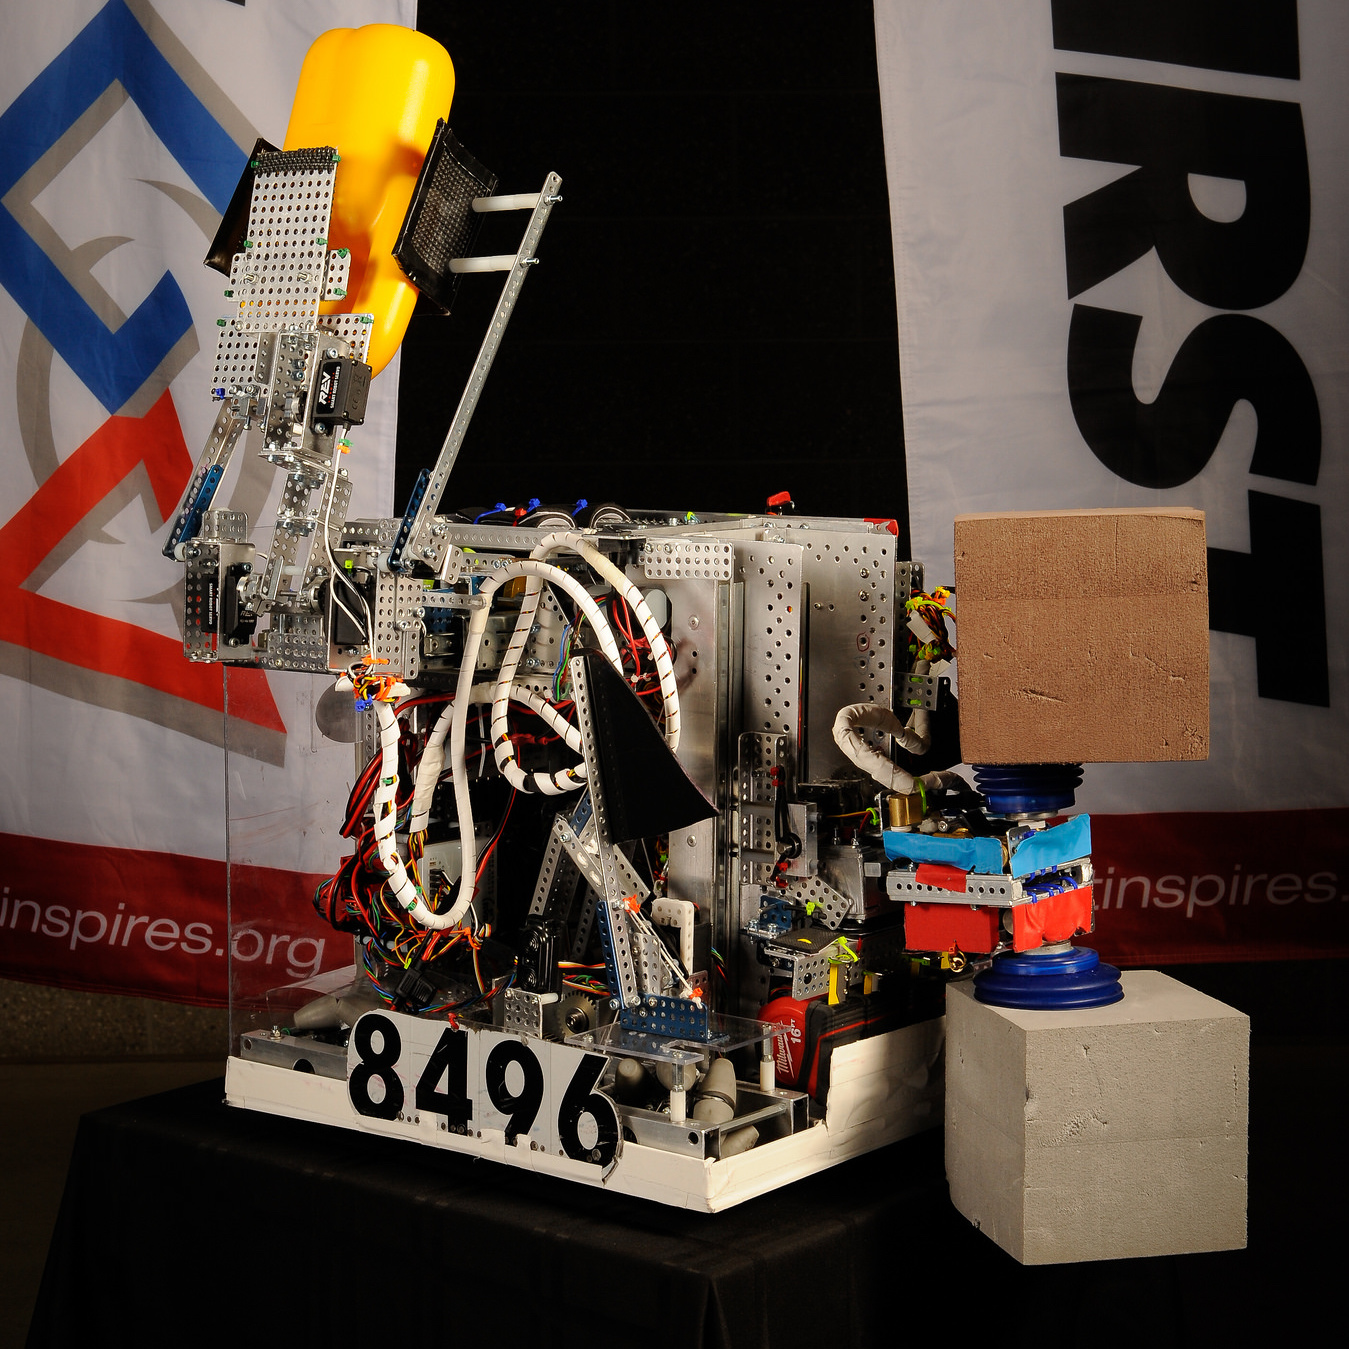
\includegraphics[width=.7\textwidth]{8496_innovate}
    \end{center}
  \end{frame}

  \begin{frame}{Design}
    \begin{itemize}
    \item Engineering section in your notebook \textbf{with detailed drawings}  (\textbf{Required})\pause
    \item Basis for design is well considered (Process counts!) \pause
    \item Robot considers both form and function \pause
    \item Robot should be well constructed
    \end{itemize}
  \end{frame}

  \begin{frame}{Design - [Team]}
  \end{frame}

  \begin{frame}{Motivate}
    \begin{itemize}
    \item Business or Strategic Plan in your notebook (\textbf{Required})\pause
    \item Promote \textit{FIRST} outside of the engineering community \pause
    \item Help grow \textit{FIRST} -- could be FLL, FTC, FRC, volunteers \pause
    \item Everybody on the team should participate
    \end{itemize}
  \end{frame}


  \begin{frame}{Motivate - 8496}
  \end{frame}

  \begin{frame}{Movivate vs. Connect}
    \[
    \begin{tabular}{r|c|c}
       & \textbf{Connect} & \textbf{Motivate} \\ \hline
      \textbf{Outreach} & Engineering Community & Non-STEM Community \\ \hline
      \textbf{Education} & Learning & Teaching \\
      \hline
    \end{tabular}
    \]
  \end{frame}

  \begin{frame}{Control}
    \begin{itemize}
    \item \textbf{FILL OUT THE CONTROL FORM} (\textbf{Required})\pause
    \item Engineering notebook should describe control system again \pause
      (should be distinct from control form) (\textbf{Required})\pause
    \item Control components should make the robot work better
    \end{itemize}
  \end{frame}

  \begin{frame}{Control, continued}
    \begin{itemize}
    \item It's not an autonomous scoring contest \pause
    \item Judge's first pass is your control form \pause
    \item Doing something interesting with sensors or algorithms
      is better than always scoring maximum points. \pause
    \item Show us that you've learned how to make the computer do
      something new
    \end{itemize}
  \end{frame}

  \begin{frame}{Control - [Team]}
  \end{frame}

  \begin{frame}{Inspire}
    \begin{itemize}
    \item Notebook must be very strong \pause
    \item Excel in both technical and non-technical categories \pause
    \item Excel in \textbf{all} categories to be sure \pause
    \item It takes much more work than you'd expect
    \end{itemize}
  \end{frame}

  \begin{frame}{Inspire}
    \begin{center}
      \begin{figure}
        \includegraphics[width=.8\textwidth]{awards_4628}
        \caption{teams with missing dimensions are unlikely to win Inspire}
        \label{}
      \end{figure}
    \end{center}
  \end{frame}

  \begin{frame}{Inspire}
    \begin{center}
      \begin{figure}
        \includegraphics[width=.8\textwidth]{awards_inspire}
        \caption{A potential Inspire nominee}
      \end{figure}
    \end{center}
  \end{frame}

  \begin{frame}{Inspire}
    \begin{center}
      \begin{figure}
        \includegraphics[width=.8\textwidth]{awards_strong_inspire}
        \caption{A likely Inspire winner}
      \end{figure}
    \end{center}
  \end{frame}

  \begin{frame}{Inspire}
    \begin{center}
      \begin{figure}
        \includegraphics[width=.8\textwidth]{awards_8496}
        \caption{Teams at the very top level}
      \end{figure}
    \end{center}
  \end{frame}

  \begin{frame}{In Conclusion...}
    \begin{itemize}
    \item{Read the game manual, do the things it says to do}
    \item{Awards are based on what you've done \textbf{and} how you present it}
    \item{Don't forget the \textbf{Required} components}
    \end{itemize}
  \end{frame}

  \begin{frame}{Thank you}
    If you have further questions:
    \begin{itemize}
    \item \texttt{cp@suitbots.com}
    \end{itemize}
  \end{frame}
\end{document}
